
\chapter{The IPFS Stack}
The IPFS stack has 6 layers as follows (bottom-up):

\begin{enumerate}
    \item Network
    \item Routing
    \item Exchange
    \item MerkleDAG
    \item Naming
    \item Application
\end{enumerate}

The MerkleDAG layer is the most important out of these. It forms a thin waist model where layers above and below it can be developed independent of each other i.e the protocols in the bottom layers can change without the upper layers knowing. Due to this independence, the layers of IPFS are being built as separate projects.

The network, routing and exchange layers are being built under a project named \textit{libp2p}\cite{libp2p}.

The merkledag layer is being built as a project named the \textit{InterPlanetary Linked Data (IPLD)}\cite{ipld}.

The naming layer is being built as a project named the \textit{InterPlanetary Naming System (IPNS)}.


\section{libp2p}

\subsection{Network Layer}
This is the lowest layer and is built mostly from existing networks protocol for reliable transfer of data. 
\subsection{Routing Layer}
The routing layer is used when we need to find which peers contain data corresponding to a particular hash value on IPFS. This requires the use of distributed hash tables.

A distributed hash table (DHT) is a lookup service similar to hash tables i.e. they store (key, value) pairs and any node in the system can efficiently give a value corresponding to any key by interacting with other nodes in the system. They differ from hash tables in that none of the nodes store the entire hash table, but only a small portion of it. The protocols for who stores which key and what is stored as a value varies between different DHTs.

IPFS used ideas from the Kademlia DHT\cite{Maymounkov:2002:KPI:646334.687801} and the Coral DHT\cite{Freedman:2004:DCP:1251175.1251193}.

Now, DHTs are an important component of p2p systems. Let's see how these systems work:

\begin{enumerate}
    \item Each node which is a part of the p2p system is given a NodeID.
    \item Kademlia stores the values in nodes which are nearest to the key. The distance is defined as the XOR of the key value and the NodeID.
    \item Every node also stores the addresses of nodes at exponentially increasing distance from itself i.e. node at distance $2^0$, $2^1$, $2^2$ and so on. Thus it stores addresses to at most $log_2(n)$ nodes where $n$ is the total number of nodes in the system. Lets call these the neighbours of a node.
    \item When a node needs to find the value corresponding to a certain key, it checks which nodeID, say $nid$, would be closest to the particular key and then looks for the node with nodeID $nid$.
    \item If the node it is looking for is one of its neighbours, it is done and can communicate directly with it to get the value corresponding to the key.
    \item If not, then it find the neighbour nearest to the node with nodeID $nid$ (can be again done using XOR distance). We'll call this neighbour $n$
    \item The node asks neighbour $n$ if it knows the address of node with nodeID $nid$.
    \item If $n$ knows the address, it returns it, otherwise returns the address of it's own neighbour closest to nodeID $nid$, say $n2$
    \item Now the node makes a query to $n2$ and the process continues. This iterative process is similar to what happens in iterative DNS.
    \item When the correct node is finally found, a query is made to it to retrieve the value corresponding to the key.
\end{enumerate}

Using the above protocol, Kademlia does an efficient lookup through massive networks by querying a maximum of $log_2(n)$ nodes. S/Kademlia also provides resistance to Sybil attacks and a low coordination overhead. It is used in systems like Gnutella and BitTorrent.

S/Kademlia\cite{Pecori:2016:SKA:2884080.2884249} also extends Kademlia to lookup values over disjoint paths so that even in the presence of a lot of adversaries, honest nodes can connect to each other.

IPFS also uses ideas from Coral DSHT (Distributed Sloppy Hash Table) to prevent hot-spots (overcrowding of all the nearest nodes when a key become popular). Coral also prevents "near" nodes from storing the data they don't need/want when "far" nodes are already storing it. To do this, the DHT stores the address of nodes containing values of a particular key rather than the value itself. Thus when the correct node is found using the above algorithm, it returns the address of all the other nodes which store that value. A query can now be made to one of these nodes to retrieve the value.


In IPFS, nodes are identified by a NodeId, the cryptographic hash
of a public-key, created with the static crypto puz-
zle used in S/Kademlia. The identity generation uses the following method:

\begin{minted}{c}
difficulty = <integer parameter>
n = Node{}
do {
    n.PubKey, n.PrivKey = PKI.genKeyPair()
    n.NodeId = hash(n.PubKey)
    p = count_preceding_zero_bits(hash(n.NodeId))
} while (p < difficulty)
\end{minted}

The interface used by IPFS's DHT is as follows:

\begin{minted}{go}
type IPFSRouting interface {
    FindPeer(node NodeId)
    // gets a particular peer's network address
    SetValue(key []bytes, value []bytes)
    // stores a small metadata value in DHT
    GetValue(key []bytes)
    // retrieves small metadata value from DHT
    ProvideValue(key Multihash)
    // announces this node can serve a large value
    FindValuePeers(key Multihash, min int)
    // gets a number of peers serving a large value
}
\end{minted}



\subsection{Exchange Layer}

This layer is built to achieve interchange of data blocks between the nodes in the p2p system. For this, IPFS takes inspiration from BitTorrent\cite{Pouwelse:2005:BPF:2138958.2138984}.

BitTorrent has some very useful features like sending the rarest pieces of data first so the non-seed peers can trade with each other. It also rewards nodes who share data and contributes to the system while punishing ones which only leech resources.



Taking the above ideas, IPFS built it's own protocol known as BitSwap. The nodes have a \textit{want\_list} and a \textit{have\_list}. The \textit{want\_list} stores which blocks the nodes is looking to acquire and the \textit{have\_list} store the blocks that it is willing to share. BitSwap forms a kind of credit system to incentivize nodes to seed even when they do not need anything in particular. This credit score also incentivizes the nodes to find, cache and distribute rare pieces of data even if doesn't want them itself.

\subsubsection{BitSwap Credit}

In BitSwap, nodes sending and receiving data from other nodes track their balance with the other node. This causes nodes to share data in the present and hoping to have the debt repaid in the future when they need data.

The data is sent with a certain probability which depends on how much debt the receiver has with that sender. As the debt increases, the probability of receiving data decreases. After every denied request the peer is ignored for an \textit{ignore\_cooldown} timeout to prevent the peer from gaming the probability by just sending a lot of requests (more dice-rolls).

\subsubsection{BitSwap Strategy}

BitSwap aims to be harsh to leechers and lenient to trusted peers even when they are temporarily unable to share data. The current algorithm:

\begin{enumerate}
    \item The node calculates a value named \textit{debt ratio} $r$ between a node and it's peer.\\
    \begin{center}\Large
        $r = \frac{bytes\_sent (in past)}{bytes\_recv (in past) + 1}$
    \end{center}
    
    
    \item Given the \textit{debt ratio} $r$, the probability of sending to a debter is given as: \\
    \begin{center}\Large
        $P(\text{send} | r) = 1 - \frac{1}{1 + \exp{6 - 3r}}$
    \end{center}
    
\end{enumerate}

A lower debt ratio means high probability of getting the data.

This method has certain other advantages as well:
\begin{enumerate}
    \item It prevents Sybil attacks since newly created nodes would all have shared no data in the past
    \item It protect nodes who have previously shared a lot of data but are temporarily unable to do so
\end{enumerate}

\subsubsection{BitSwap Ledger}

The data needed to calculate the debt ratio needs to be stored somewhere. Each node stores a \textit{Ledger} to keep track of exchange with all the other nodes.

The \textit{Ledger} structure looks as follows:

\begin{minted}{c}
type Ledger struct {
    owner NodeId
    partner NodeId
    bytes_sent int
    bytes_recv int
    timestamp Timestamp
}
\end{minted}

This ledger is sent to the peer while requesting information. If the data inside the ledger does not exactly match what the peer has, the ledger is re-initialized to zero. A node may try to lose the debt by sending a random ledger, but they would also lose the acquired credit so there is a trade-of.

\subsubsection{BitSwap Interface}

The BitSwap protocol has the following interface:

\begin{minted}{go}
// Protocol interface:
interface Peer {
    open (nodeid :NodeId, ledger :Ledger);
    send_want_list (want_list :WantList);
    send_block (block :Block) -> (complete :Bool);
    close (final :Bool);
}
\end{minted}

\begin{enumerate}
    \item open (nodeid :NodeId, ledger :Ledger) : This function is used to open a connection with a peer a node wants data from. The node send the ledger corresponding to that peer in the request. The peer can choose to accept or reject the connection based on the debt of the node or the values in the ledger.
    \item send\_wan\_list (want\_list :WantList) : After the connections has opened, the node sends its want list to the peer. The peer checks if it has any of the wanted blocks and then sends it according to the BitSwap strategy.
    \item send\_block (block :Block) : This is used by the peer to send the requested block to the node. After the node has received all the data, the node calculates the multihash checksum to see it if indeed received the correct data. If the block is accepted it moves from the want\_list to have\_list. The ledgers are updated accordingly.
    \item close (final :Bool) : This is used to close the connection after the block has been received from the peer (or in case of a timeout).
\end{enumerate}
\section{IPLD - Creating the merkle forest}

The InterPlanetary Linked Data (IPLD) is at the core of IPFS. It emerges as a direct result of trying to make the web content-addressable. It allows the treatment of all hash-linked data structures under a single category. Thus any data model which links data using hashes can be treated as an instance of IPLD. Example of technologies using such data structures are git, Bitcoin, Ethereum and now IPFS. With IPLD, links can be traversed across protocols boundaries.

\subsection{MerkleDAG}

IPLD is based on the concept of MerkleDAGs, which are directed acyclic graphs where links between objects are cryptographic hashes of the targets embedded in the sources. It is inspired from the Git data structures but does make some modifications to it.

This allows for many useful properties like:
\begin{enumerate}
    \item \textbf{Integrity}: The hashes act as checksums to make sure that the data you get is the one you requested
    \item \textbf{Deduplication}: Different files can have certain blocks of data which are same. Since these blocks have the same hash, they only need to be stored once.
    \item \textbf{Content Addressibility}: Since the hashes are cryptographic, all content can be uniquely identified by their hash
\end{enumerate}

\section{Versioned File System}

\begin{figure}[h]
\caption{Sample object graph}
\centering
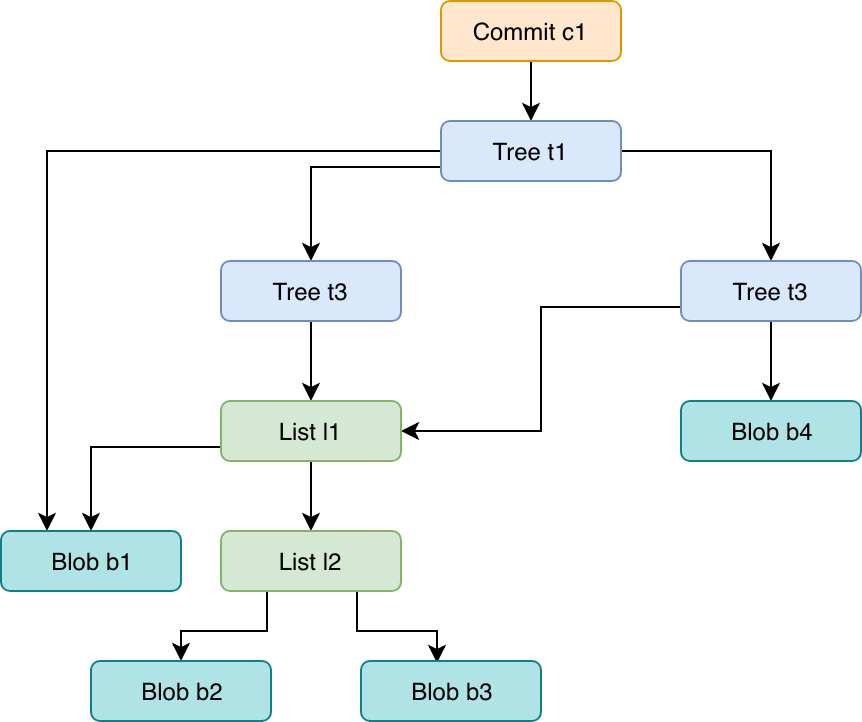
\includegraphics[width=0.5\textwidth]{ipfs}
\end{figure}


IPFS defines a set of objects, inspired from git, to allow a versioned file system on top of the MerkleDAG. These objects are as follows:

\begin{enumerate}
    \item \textbf{blob}: A blob is just raw data which is content-addressible.It does not link to anything else.
    \begin{minted}{c}
    {
        "data": "some data here",
        // blobs have no links
    }
    \end{minted}
    \item \textbf{list}: Lists are not present in git and is something that IPFS has introduced. It is used to represent a large or deduplicated file which has been broken into various pieces. Lists can have other lists or blobs inside them. The order in which the blobs or lists occur is important. This also allows in-file deduplication i.e. when blobs in the file have the exact same data. In addition to links, a list also stores the size of content referred by the link. This helps in making size calculations easier.
    
    \begin{minted}{c}
    {
        "data": ["blob", "list", "blob"],
        // lists have an array of object types as data
        "links": [
        { "hash": "QmcCcJMotPnNS8dUbybG7vH32u27smnCfrYWWhazyKMT18",
        "size": 9458 },
        { "hash": "QmRjRnx15pXLKbXz3y62wsJarDRGdrhDbu3AZUQmhqgugh",
        "size": 19441 },
        { "hash": "QmRy2xuqAgJxThesKFBMosAne6rxPKbmYNYkYJZwnsXgiE",
        "size": 5286 }
        // lists have no names in links
        ]
    }
    \end{minted}
    \item \textbf{tree}: Trees are used to map names to hashes. They represent directories. They can link to blobs, lists, other trees and commits. The names help in path resolution.
    \begin{minted}{c}
    {
        "data": ["blob", "list", "blob"],
        // lists have an array of object types as data
        "links": [
        { "hash": "QmcCcJMotPnNS8dUbybG7vH32u27smnCfrYWWhazyKMT18",
        "name": "hello", "size": 9458 },
        { "hash": "QmRjRnx15pXLKbXz3y62wsJarDRGdrhDbu3AZUQmhqgugh",
        "name": "demo", "size": 19441 },
        { "hash": "QmRy2xuqAgJxThesKFBMosAne6rxPKbmYNYkYJZwnsXgiE",
        "name": "world", "size": 5286 }
        // trees do have names for links
        ]
    }
    \end{minted}
    \item \textbf{commit}: A commit represents the version history of an object. It links to previous commit as well as the objects in the new commit. It also stores additional information like commit message, link to author etc.
    \begin{minted}{c}
    {
        "data": {
            "type": "tree",
            "date": "2018-11-2 12:20:00Z",
            "message": "This is a commit message."
        },
        "links": [
        { "hash": "QmcCcJMotPnNS8dUbybG7vH32u27smnCfrYWWhazyKMT18",
        "name": "parent", "size": 21309 },
        { "hash": "QmRjRnx15pXLKbXz3y62wsJarDRGdrhDbu3AZUQmhqgugh",
        "name": "object", "size": 4568 },
        { "hash": "QmRy2xuqAgJxThesKFBMosAne6rxPKbmYNYkYJZwnsXgiE",
        "name": "author", "size": 120 }
        ]
    }
    \end{minted}
\end{enumerate}

\subsection{Content Addressing}

The way in which the above objects are defined makes it very easy to address a particular object as well as traverse through the merkledag.

The path format for IPFS is as follow:
\begin{minted}{text}
    /ipfs/<hash-of-object>/<name-path-to-object>
\end{minted}
The hash of the object retrieves the object and then the links inside the objects are followed according to the name-path mentioned. This allow for multiple ways to access a file. For example, given three objects in path
<foo>/bar/baz, the last object is accessible by all:

\begin{minted}{text}
    /ipfs/<hash-of-foo>/bar/baz
    /ipfs/<hash-of-bar>/baz
    /ipfs/<hash-of-baz>
\end{minted}

\subsection{Splitting files}
When a file is being added to IPFS, it needs to be broken into blobs and lists. Finding the optimal way to break the file is a hard problems and depends on many factors including what all blocks are already present in the system. IPFS allows users to define their own block splitting methods specific to files.

\subsection{The Merkle Forest}
IPFS is like a forest of linked merkleDAGs since it allows systems like ethereum, bitcoin, git to interoperate. Some sample uses of this could be:

\begin{enumerate}
    \item Referencing a commit in bitcoin to timestamp it - Using IPLD would allow us to transparently traverse from the bitcoin transaction into the files present in the commit.
    \item Store Ethereum media on IPFS: Using IPLD would allow seamless jumping from the Ethereum contract or transaction to the media.
\end{enumerate}


\subsection{Multiformats}
Multiformats is a project to create self-describing values which means that looking at the value helps you understand how it was obtained and how you can process it. It includes multiple subprojects namely multihash, multicodec, multibase, multiaddr, multikey and multistream.

Lets take the example of hashes. Based on which has we are using, the same content can hash to different values. Now, only by looking at the hash value, you cannot know which hash function was used. That is where multihashes come in. Multihashes have a hash function code and hash length appended to them at the beginning. The format is as follows:

\begin{minted}{text}
    <fn-code><hash length><hash>
\end{minted}

This is the reason why, by default, IPFS hashes start with \textit{Qm}.

\section{IPNS - Naming the data}

As we discussed immutable paths provide various benefits to IPFS like integrity checking and indefinite caching (If you know an object is not going to change it's cache need not expire ever).

But this implies that if an object is changed, then the new IPFS link needs to be sent to people who want to access it. Thus we need some way to retrieve mutable state at the same path. This is where InterPlanetary Naming System (IPNS) comes in.

\subsection{Self-certified Names}
IPFS uses the naming scheme from SFS \cite{Mazieres:2000:SFS:934196} to construct a mutable namespace for every node. These names are self-certified, which means that the information used to retrieve the actual data is signed by the private key of the node. This provides a guarantee that the data indeed belongs to that node.

In IPFS, $NodeID = hash(node.PubKey)$ and each user gets a mutable namespace at
\begin{minted}{text}
    /ipns/<NodeID>
\end{minted}

Now since everything in IPFS is content addressed, we need a way to go from an IPNS address to an actual IPFS address. The Routing system comes to rescue here.

The first step is to publish the object in a regular manner and get it's IPFS address. Then we publish this hash on the routing system as a metadata value with the NodeId as the key.

\begin{minted}{c}
    routing.setValue(NodeId, <ns-object-hash>)
    // Here NodeId is the IPNS address of the object
\end{minted}

This mapping can be changed by the private key holder in the future, thus allowing the same name to point to different things at different time.

\subsection{Human Readable Names}
We can see that IPNS names are hard to remember and not very user friendly.

One of the ways in which IPFS solves this problem (especially useful for websites hosted on IPFS) is to allow ipfs and ipns address in the DNS TXT records.

An example of a TXT record in my own website is as follow:

\begin{minted}{c}
    ee465.akashtrehan.com.  1799    IN  TXT
    "dnslink=/ipns/QmWBPZZ59ZDgigAthNEa2sjuiDTKbRdaBjVYDH4tfZHdHS"
\end{minted}

On requesting the location,

\begin{minted}{text}
    /ipns/ee465.akashtrehan.com
\end{minted}

IPFS first looks up the TXT DNS records for \textit{ee465.akashtrehan.com}, then looks for the record with a \textit{dnslink}.

It then "redirects" to that address mentioned in the dnslink. In this case \begin{minted}{text}
    /ipns/ee465.akashtrehan.com
\end{minted}
resolves to 

\begin{minted}{text}
    /ipns/QmWBPZZ59ZDgigAthNEa2sjuiDTKbRdaBjVYDH4tfZHdHS
\end{minted}

which further resolves to the IPFS address
\begin{minted}{text}
    /ipfs/QmYz3vZGv3gi2AYNptfYM3DxxrqkE5gbSxq1tKtiGS6DJk
\end{minted}

The content corresponding to this IPFS address is finally retrieved by the block exchange system.



% \todo{Mention bitswap here}
